% --------------------- VARIABLEN -------------------------

\newcommand{\COURSE}{Physik und Materialwissenschaften\\ Praktikum Physik \\}
\newcommand{\SEMESTER}{Elektro- und Informationstechnik II}
\newcommand{\STUDENT}{Maximilian Spahn\\ und\\Benjamin Langer}

\newcommand{\HEADDING}{Praktikum Physik}
\newcommand{\SUBHEADDING}{Versuch 2.2: Stehende Wellen und Beugung am Doppelspalt}

% ------------------- DEFINITIONEN -----------------------

\documentclass[a4paper]{scrartcl}

\usepackage[utf8]{inputenc}
\usepackage[ngerman]{babel}
\usepackage{amsmath}
\usepackage{amssymb}
\usepackage{color}
\usepackage{tikz}
\usepackage{float}
\usetikzlibrary{arrows,decorations.markings}
\usepackage{tabularx}
\usepackage{fancybox}
\usepackage{pgfplots}
\usepackage{geometry}
\usepackage{fancyhdr}
\usepackage[page]{totalcount}
\usepackage[colorlinks=true,linkcolor=black,urlcolor=blue,bookmarks,bookmarksopen=true]{hyperref}

%Größe der Ränder setzen
\geometry{a4paper,left=2cm, right=2cm, top=3cm, bottom=2cm, headheight=8cm}

%Kopf- und Fußzeile
\pagestyle {fancy}
\fancyhf{}
\fancyhead[L]{\STUDENT}
\fancyhead[C]{\COURSE}
\fancyhead[R]{\today}

\fancyfoot[L]{\SEMESTER}
\fancyfoot[C]{}
\fancyfoot[R]{Seite \thepage /\pageref{LastPage}}

%Formatierung der Überschrift, hier nichts ändern
\def\header#1#2{
  \begin{center}
    {\Large #1}\\
    {#2}
  \end{center}
}

\numberwithin{equation}{subsection}

\setlength\parindent{0pt}

% ----------------------- DOCUMENT ---------------------------

\begin{document}

\vspace{10pt}
\header{\HEADDING}{\SUBHEADDING}

\tableofcontents

\newpage

\section{Einleitung}
\subsection{Stehende Wellen}
Bei diesem Versuch soll die Intensität in Abhängigkeit vom Abstand in ein Diagramm eingetragen werden. Dadurch lassen sich im Diagramm die charakteristischen Eigenschaften einer Stehenden Welle erkennen.
\subsection{Beugung am Doppelspalt}
Der Versuch handelt sowohl von der messtechnischen als auch der theoretischen Bestimmung der Maxima und Minima bei Beugung einer Welle am Doppelspalt. Dafür wird die Intensität in Abhängigkeit vom Beugungswinkel gemessen.

\newpage

\section{Theorie}
Periodische Zustandsänderungen zwischen zwei oder mehreren Zuständen, nennt man Schwingungen. [3]
Dabei wird Energie wird zwischen Energiereservoirs periodisch hin- und herbewegt, wodurch die Schwingung entsteht.
Meist wird eine einmalige Energie, in Form von elektrischer oder
mechanischer Energie zugeführt und anschließend das System sich selbst überlassen, wodurch eine sogenannte freie Schwingung entsteht. [2]

\subsection{Mechanischer Oszillator}
Am einfachsten lassen sich Schwingungen an einem mechanischen Oszillator, wie in diesem Fall einem Federpendel (im Versuch ein Rotationsschwinger), erläutern. Ein Feder-Masse-Schwinger besteht aus einer Masse auf einer waagrechten, reibungsfreien Unterlage, welche an einer Feder befestigt ist. Dabei wird die potenzielle Energie der Feder in die kinetische Energie der Masse und umgekehrt gewandelt [3].

%\begin{figure}[H]
%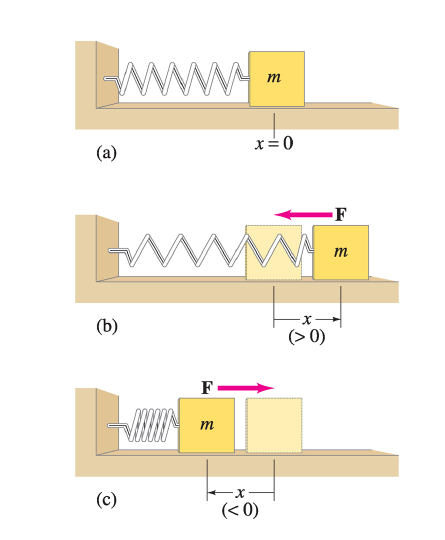
\includegraphics[width=4cm]{Grafik_Federpendel}
%\centering
%\caption{Federpendel [1]}
%\centering
%\end{figure}

Wird die Masse wie zuvor beschrieben ausgelenkt, also Energie zugeführt, und anschließend losgelassen, so schwingt das System um den Grundzustand. 
Über die Zeit betrachtet, führt die Masse eine Sinusschwingung aus, mit welcher sich allgemein Schwingungen beschreiben lassen:

\begin{align}
y(t) = \widehat{y} = sin(\omega_0 t )
\end{align}


Dabei ist $\widehat{y}$ die Amplitude, also die Auslenkung der Schwingung und $\omega_0$ die Kreisfrequenz mit welcher das System schwingt. 
Diese Berechnet sich aus der Frequenz, bzw. der Periodendauer [3]:

\begin{align}
T = \frac{1}{f}
\omega_0 = 2\pi \cdot f = \frac{2\pi}{T}
\end{align}

Für jedes schwingende System lässt sich eine Differentialgleichung aufstellen, mit welchem sich die verschiedenen wirkenden Kräfte beschreiben lassen. Für das lineare Feder-Masse-System ohne Dämpfung gilt: [2]

\begin{align}
F_a &= F_k &\\
\text{nach dem 2. Newtonsche Axiom gilt für die Masse:} F_a &= m \cdot a &\\
\text{und für die Federkraft das Hookesches Gesetz:} F_k &= -k \cdot y &
\end{align}

Durch einsetzen erhält man ein Gleichungssystem:

\begin{align}
-ky &= ma \\
m \frac{\partial y}{\partial t} + ky &= 0
\end{align}

Mit dem Ansatz $y(t) = \widehat{y_0} \cdot cos(\omega_0 t + \varphi_0)$ ergibt sich für das DGL.:

\begin{align}
\omega_0 = \sqrt{\dfrac{k}{m}}
\end{align}

Bei dem vorherigen System handelt es sich um eine freie ungedämpfe Schwingung. Diese gibt es in der Realität nur selten. Darum wird als nächstes die freie, gedämpfte Schwingung betrachtet.
Bei dieser wirkt eine Kraft, welche sich proportional zur Geschwindigkeit verhält und dem System Energie entzieht.

\begin{align}
F_D = -b \cdot v
\end{align}

Dabei ist b die Dämpfungskonstante. \\ 
Für die gedämpfte Schwingung lässt sich das DGL. um diesen Teil erweitern, wodurch sich folgendes Gleichungssystem ergibt.

\begin{align}
m \ddot{y} + d \dot{y} + k y = 0 
\end{align}

Der Ansatz für dises DGL. ist:

\begin{align}
y(t) = \widehat{y_0} e^{\delta t} cos(\omega_d t + \varphi_0)
\end{align}

Daraus als Lösung ergibt sich:

\begin{align}
\omega_d = \sqrt{\omega_0^2 - \delta^2} &\\
\delta = \dfrac{d}{2m} &\\
\omega_0 = \sqrt{\dfrac{k}{m}}
\end{align}

Dabei ist $\delta$ der Abklingkoeffizient. \\ \\

Abhängig von $\delta$ im Vergleich zu $\omega_0$ ergeben sich drei Fälle:

\textbf{Schwingfall:}\\
Wenn $\omega_0 > \delta$ schwingt das System mit abnehmender Amplitude und kann mit der Bewegungsgleichung

\begin{align}
y(t) = \widehat{y_0} e^{\delta t} cos(\omega_d t + \varphi_0)
\end{align}

beschrieben werden. [1]\\ 

\textbf{aperiodischer Genzfall:}\\
Wenn $\omega_0 = \delta$ schwingt das System nicht. Die Auslenkung strebt schnellstmöglich gegen Null. [1]\\

\textbf{Kriechfall:}\\
Wenn $\omega_0 < \delta$ schwingt das System ebenfalls nicht. Die Amplitude nimmt ganz langsam ab und erreicht asymptotisch die Null. [1]\\


Das folgende Diagramm zeigt das Verhalten bei den jeweiligen drei Fällen:

%\begin{figure}[H]
%\includegraphics[width=8cm]{Grafik_Fälle-Schwingungen}
%\centering
%\caption{Die drei Fälle der gedämpften Schwingung [1]}
%\centering
%\end{figure}

\subsection{Elektrischer Oszillator}
Der elektrische Oszillator ist dem mechanischen sehr ähnlich. Auch hier wird Ladungsenergie zwischen Kondensator und Spule stetig verschoben. Als Dämpfung wirkt der ohmsche Widerstand. 

In dem dargestellten Schwingkreis muss [3]:
\begin{align}
U_L + U_R + U_C = 0
\end{align}

Durch einsetzen der Strom- Spannungsabhängigkeiten für Widerstand, Spule und Kondensator [3]:
\begin{align}
U_L = L \cdot \frac{\partial i}{\partial t} &\\
U_C = \frac{1}{C} \cdot q &\\
U_R = R \cdot i &\\
\text{und:} \frac{\partial q}{\partial t} = i &
\end{align}

ergibt sich das DGL. [1]:
\begin{align}
L \cdot \frac{\partial^2 q}{\partial t^2} + R \cdot \frac{\partial q}{\partial t} + \frac{1}{c} \cdot q = 0
\end{align}

dessen Lösungen sind analog zu der mechanischen Schwingung [1]:
\begin{align}
\omega_d = \sqrt{\omega_0^2 - \delta^2} &\\
\delta = \dfrac{R}{2L} &\\
\omega_0 = \sqrt{\dfrac{1}{L \cdot C}}
\end{align}

\newpage

\section{Häusliche Vorarbeit}
\subsection{Stehende Wellen}
\subsubsection[Berechnen von Gleichung 7 aus 6]{Berechnen von Gleichung 7 aus 6 \footnote{Die Bezeichnungen der Gleichungen stammen aus dem Skript \glqq Versuch 2.2 - Stehende Wellen und Beugung am Doppelspalt\grqq}}

\begin{align}
\label{eq:StehendeWelle}
A_{\text{res}} = A_{\text{in}} + A_{\text{refl}} = A_0sin(\omega t-k_xx)+A_0sin(\omega t+k_xx)\qquad (6)
\end{align}
mit
\begin{align*}
k_x\quad &\text{Wellenzahl}&&k_x=\frac{2\pi}{\lambda}&\\
\omega \quad&\text{Kreisfrequenz}&&\omega=2\pi f=\frac{2\pi}{T}&\\
T\quad&\text{Periodendauer}&\\
A_{0}\quad&\text{Amplitude}&\\
x\quad&\text{Ort}&\\
y\quad&\text{Zeit}&\\
\end{align*}
Wir benötigen folgendes Additionstheorem, um die Gleichung zu vereinfachen:
\begin{align}
\label{eq:Additionstheorem}
sin(x_1+x_2)+sin(x_1-x_2)=2sin(x_1)\cdot cos(x_2)\qquad [5]
\end{align}
Nach Anwendung des Additionstheorems (Gleichung \ref{eq:Additionstheorem}) auf Gleichung \ref{eq:StehendeWelle} vereinfacht sich die Gleichung:
\begin{align}
A_{\text{res}}=2A_0sin(\omega t)\cdot cos(k_xx) \qquad (7)
\end{align}

\subsubsection{Stehende Welle zu verschiedenen Zeitpunkten innerhalb einer Periode skizzieren}
Um eine stehende Welle zu acht verschiedenen Zeitpunkten innerhalb einer Periode zu skizzieren, wird ein regelmäßiger Abstand von $\frac{1}{8}T$ gewählt. Diese acht Zeiten werden in die Gleichung 3.1.3 eingesetzt. Dadurch erhält man eine Gleichung, welche nur von $x$ abhängig ist, die sich leicht skizzieren lässt.\\\\
Wenn man sich die acht Skizzen in Abbildung~\ref{fig:skizzeStehendeWelle} anschaut, erkennt man eine stehende Welle, bei der sich die Amplitude in abhängigkeit der Zeit verändert. Es verändern sich nur die Berge (Maxima) und Täler (Minima), die Knoten (Wendepunkte) bleiben dabei an der selben Stelle.

\begin{figure}[H]
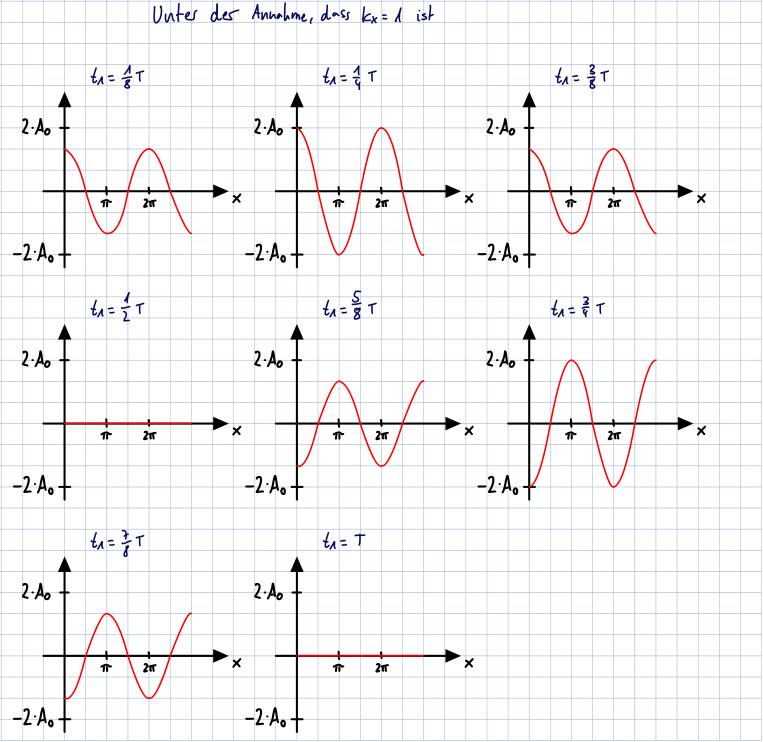
\includegraphics[width=12cm]{Skizze_Stehende_Welle}
\centering
\caption{Skizze - $A_{\text{res}}(x,t)$ für verschiedene Zeitpunkte $t$}
\centering
\label{fig:skizzeStehendeWelle}
\end{figure}

\subsubsection{Vergleich $A_{\text{res}}(x,t)$ und $A_{\text{res}}^2(x,t)$ im Bezug auf die Wellenlänge}
\label{sec:Faktor4}
Durch das Quadrieren einer Funktion, verdoppelt sich die Frequenz. (siehe Abbildung~\ref{fig:skizzeStehendeWelleQ}) Dadurch ist die Periodendauer von $A_{\text{res}}^2(x,t)$ halb so lang, wie die von $A_{\text{res}}(x,t)$. Folglich ist der Abstand zwischen zwei Maxima/Minima gleich $\frac{\lambda}{2}$.

\begin{figure}[H]
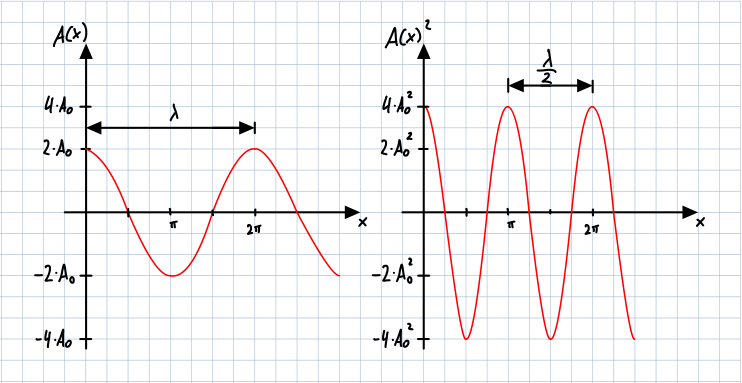
\includegraphics[width=12cm]{Skizze_Stehende_Welle_q}
\centering
\caption{Skizze - $A_{\text{res}}(x,t)$ und $A_{\text{res}}^2(x,t)$}
\centering
\label{fig:skizzeStehendeWelleQ}
\end{figure}

\subsection{Beugung am Doppelspalt}
Im folgenden Abschnitt wird die konstruktive und destruktive Interferenz am Doppelspalt hergeleitet. Dafür wird die Skizze in Abbildung~\ref{fig:skizzeDoppelspalt} verwendet.

\begin{figure}[H]
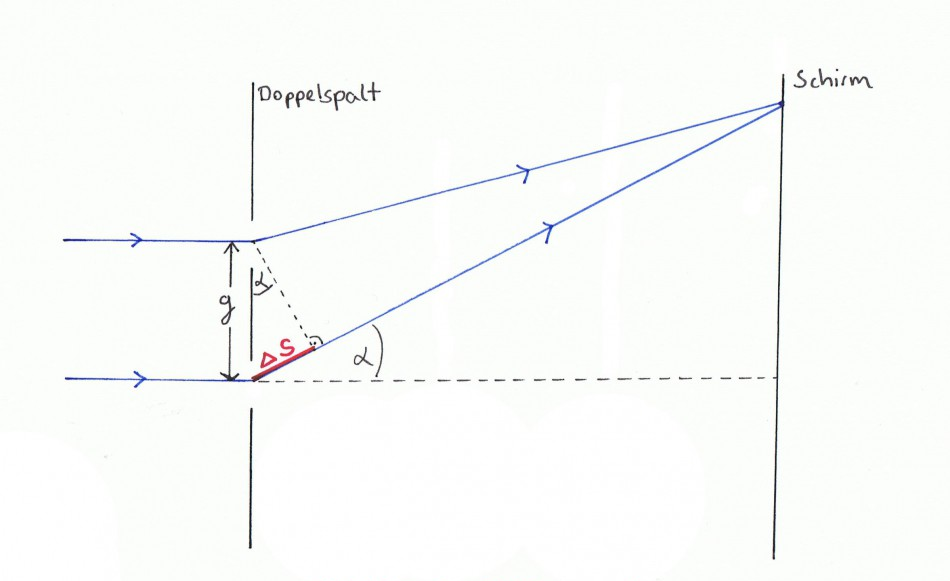
\includegraphics[width=10cm]{Skizze_Doppelspalt}
\centering
\caption{Skizze - Beugung am Doppelspalt [4]}
\centering
\label{fig:skizzeDoppelspalt}
\end{figure}

\subsubsection{Gleichung für die konstruktive Interferenz herleiten}
Um die Gleichung \ref{eq:konstruktiveInterferenz} zu verstehen, kann man einen Blick auf Abbildung \ref{fig:skizzeDoppelspalt} werfen. Alternativ kann auch die Abbildung 2(b) [1] verwendet werden.\\
Zur Herleitung der Gleichung werden die Winkelfunktionen benötigt. In diesem Fall wird die trigonometrische Funktion des Sinus verwendet:
\begin{align}
sin(x)=\frac{Gegenkathete}{Hypotenuse}
\end{align}
In unserem Fall wird für die Gegenkathete $\Delta s$ und für die Hypotenuse $d$ eingesetzt.
\begin{align}
\label{eq:deltaS}
sin(\theta)=\frac{\Delta s}{d}
\end{align}
Die Strecke $\Delta s$ beträgt bei konstruktiver Interferenz ein vielfaches der Wellenlänge $\lambda$. Setzt man nun $\Delta s = m \cdot \lambda$ in die Gleichung \ref{eq:deltaS} ein, erhält man:
\begin{align}
\label{eq:konstruktiveInterferenz}
sin(\theta)=\frac{m \cdot \lambda}{d}
\end{align}
mit
\begin{align*}
\theta \quad &\text{Beugungswinkel}&\\
d \quad &\text{Spaltabstand}&\\
m \quad &\text{Ordnung des Maximums}&\\
\end{align*}

\subsubsection{Gleichung für die destruktive Interferenz herleiten}
Es wird wieder die Abbildung \ref{fig:skizzeDoppelspalt} verwendet. Alternativ kann auch Abbildung 2(c) [1] verwendet werden.\\
Für diese Gleichung wird ebenfalls die Winkelfunktion des Sinus zur Hilfe genommen. Bei destruktiver Interferenz entspricht die Strecke $\Delta s$ nur $\frac{\lambda}{2}$. Durch einsetzen der Bedingung $\Delta s = (2m-1) \cdot \frac{\lambda}{2}$ in Gleichung \ref{eq:deltaS}, erhält man folgende Gleichung:
\begin{align}
\label{eq:destrutiveInterferenz}
sin(\theta)=\frac{(2m-1) \cdot \frac{\lambda}{2}}{d}
\end{align}
mit
\begin{align*}
\theta \quad &\text{Beugungswinkel}&\\
d \quad &\text{Spaltabstand}&\\
m \quad &\text{Ordnung des Minimums}&\\
\end{align*}

\newpage

\section{Aufbau und Durchführung}
\subsection{Stehende Wellen}
\subsubsection{Aufbau}
In Abbildung \ref{fig:AufbauStehendeWellen} ist der Versuchsaufbau dargestellt. Man benötigt einen Mikrowellensender (bestehend aus Versorgungsspannung und Hornstrahler), ein Multimeter, eine E-Feld-Sonde und eine Metallplatte, an der die Welle reflektiert wird.\\
Im Anhang finden Sie außerdem eine Skizze zum Aufbau. (Abschnitt \ref{sec:SkizzeStehendeWellen}/Abbildung \ref{fig:SkizzeStehendeWellen})

\begin{figure}[H]
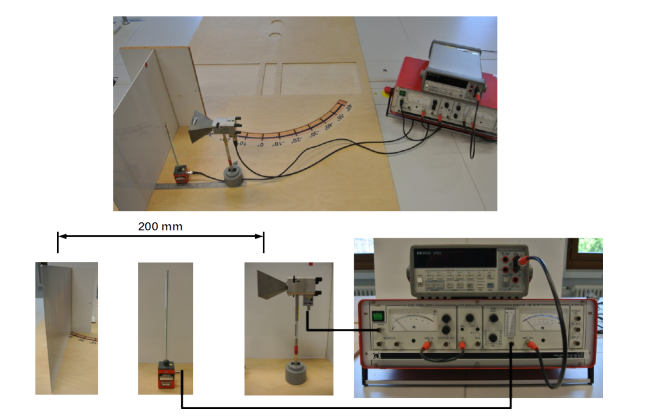
\includegraphics[width=10cm]{Aufbau_Stehende_Wellen}
\centering
\caption{Versuchsaufbau - Stehende Wellen [1]}
\centering
\label{fig:AufbauStehendeWellen}
\end{figure}

\subsubsection{Durchführung}
Zuerst wird die E-Feld-Sonde 50 mm von der Metallplatte entfernt aufgestellt. Danach wird in Schritten von 2 mm im Bereich ($50-112$) mm ein Spannungswert mit Hilfe des Multimeters gemessen.\\
Als Messunsicherheit wurde $U_s = 2$ mm angenommen.

\subsection{Beugung am Doppelspalt}
\subsubsection{Aufbau}
In Abbildung \ref{fig:AufbauDoppelspalt} ist der Versuchsaufbau dargestellt.\\
Im Anhang finden Sie außerdem eine Skizze zum Aufbau. (Abschnitt \ref{sec:SkizzeDoppelspalt}/Abbildung \ref{fig:SkizzeDoppelspalt})

\begin{figure}[H]
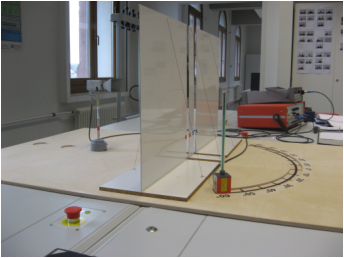
\includegraphics[width=7cm]{Aufbau_Doppelspalt}
\centering
\caption{Versuchsaufbau - Beugung am Doppelspalt [1]}
\centering
\label{fig:AufbauDoppelspalt}
\end{figure}

\subsubsection{Durchführung}
Die E-Feld-Sonde wir in einem Bereich von $+60 ^\circ$ bis $-60 ^\circ$ in $5 ^\circ$ Schritten bewegt. An jeder Stelle wurden drei Messwerte mit dem Multimeter aufgenommen.\\
Als Messunsicherheit wurde $U_\theta = 2 ^\circ$ angenommen.
\newpage

\section{Auswertung Versuch}
\label{sec:runden}
Alle Messwerte wurden mit Excel wie folgt berechnet:\\
Mittelwerte:
\begin{align}
=\text{RUNDEN}(\text{MITTELWERT}(...);\text{Anzahl Nachkommastellen})
\label{eq:mittelWert}
\end{align}
Messunsicherheit:
\begin{align}
=\frac{\text{STABW.S}(...)}{\text{WURZEL}(\text{ANZAHL}(...))} \cdot k
\label{eq:Unsicherheit}
\end{align}
mit
\begin{align*}
k \quad &\text{Erweiterungsfaktor} = 2&\\
\end{align*}
Messunsicherheiten werden immer auf zwei signifkante Stellen aufgerundet.
\subsection{Stehende Wellen}
Die Messwerte in Tabelle \ref{tab:MesswerteStehendeWellen} (Abschnitt \ref{sec:MesswerteStehendeWellen}) wurden in Abbildung \ref{fig:DiagrammStehendeWelle} graphisch dargestellt.

\begin{figure}[H]
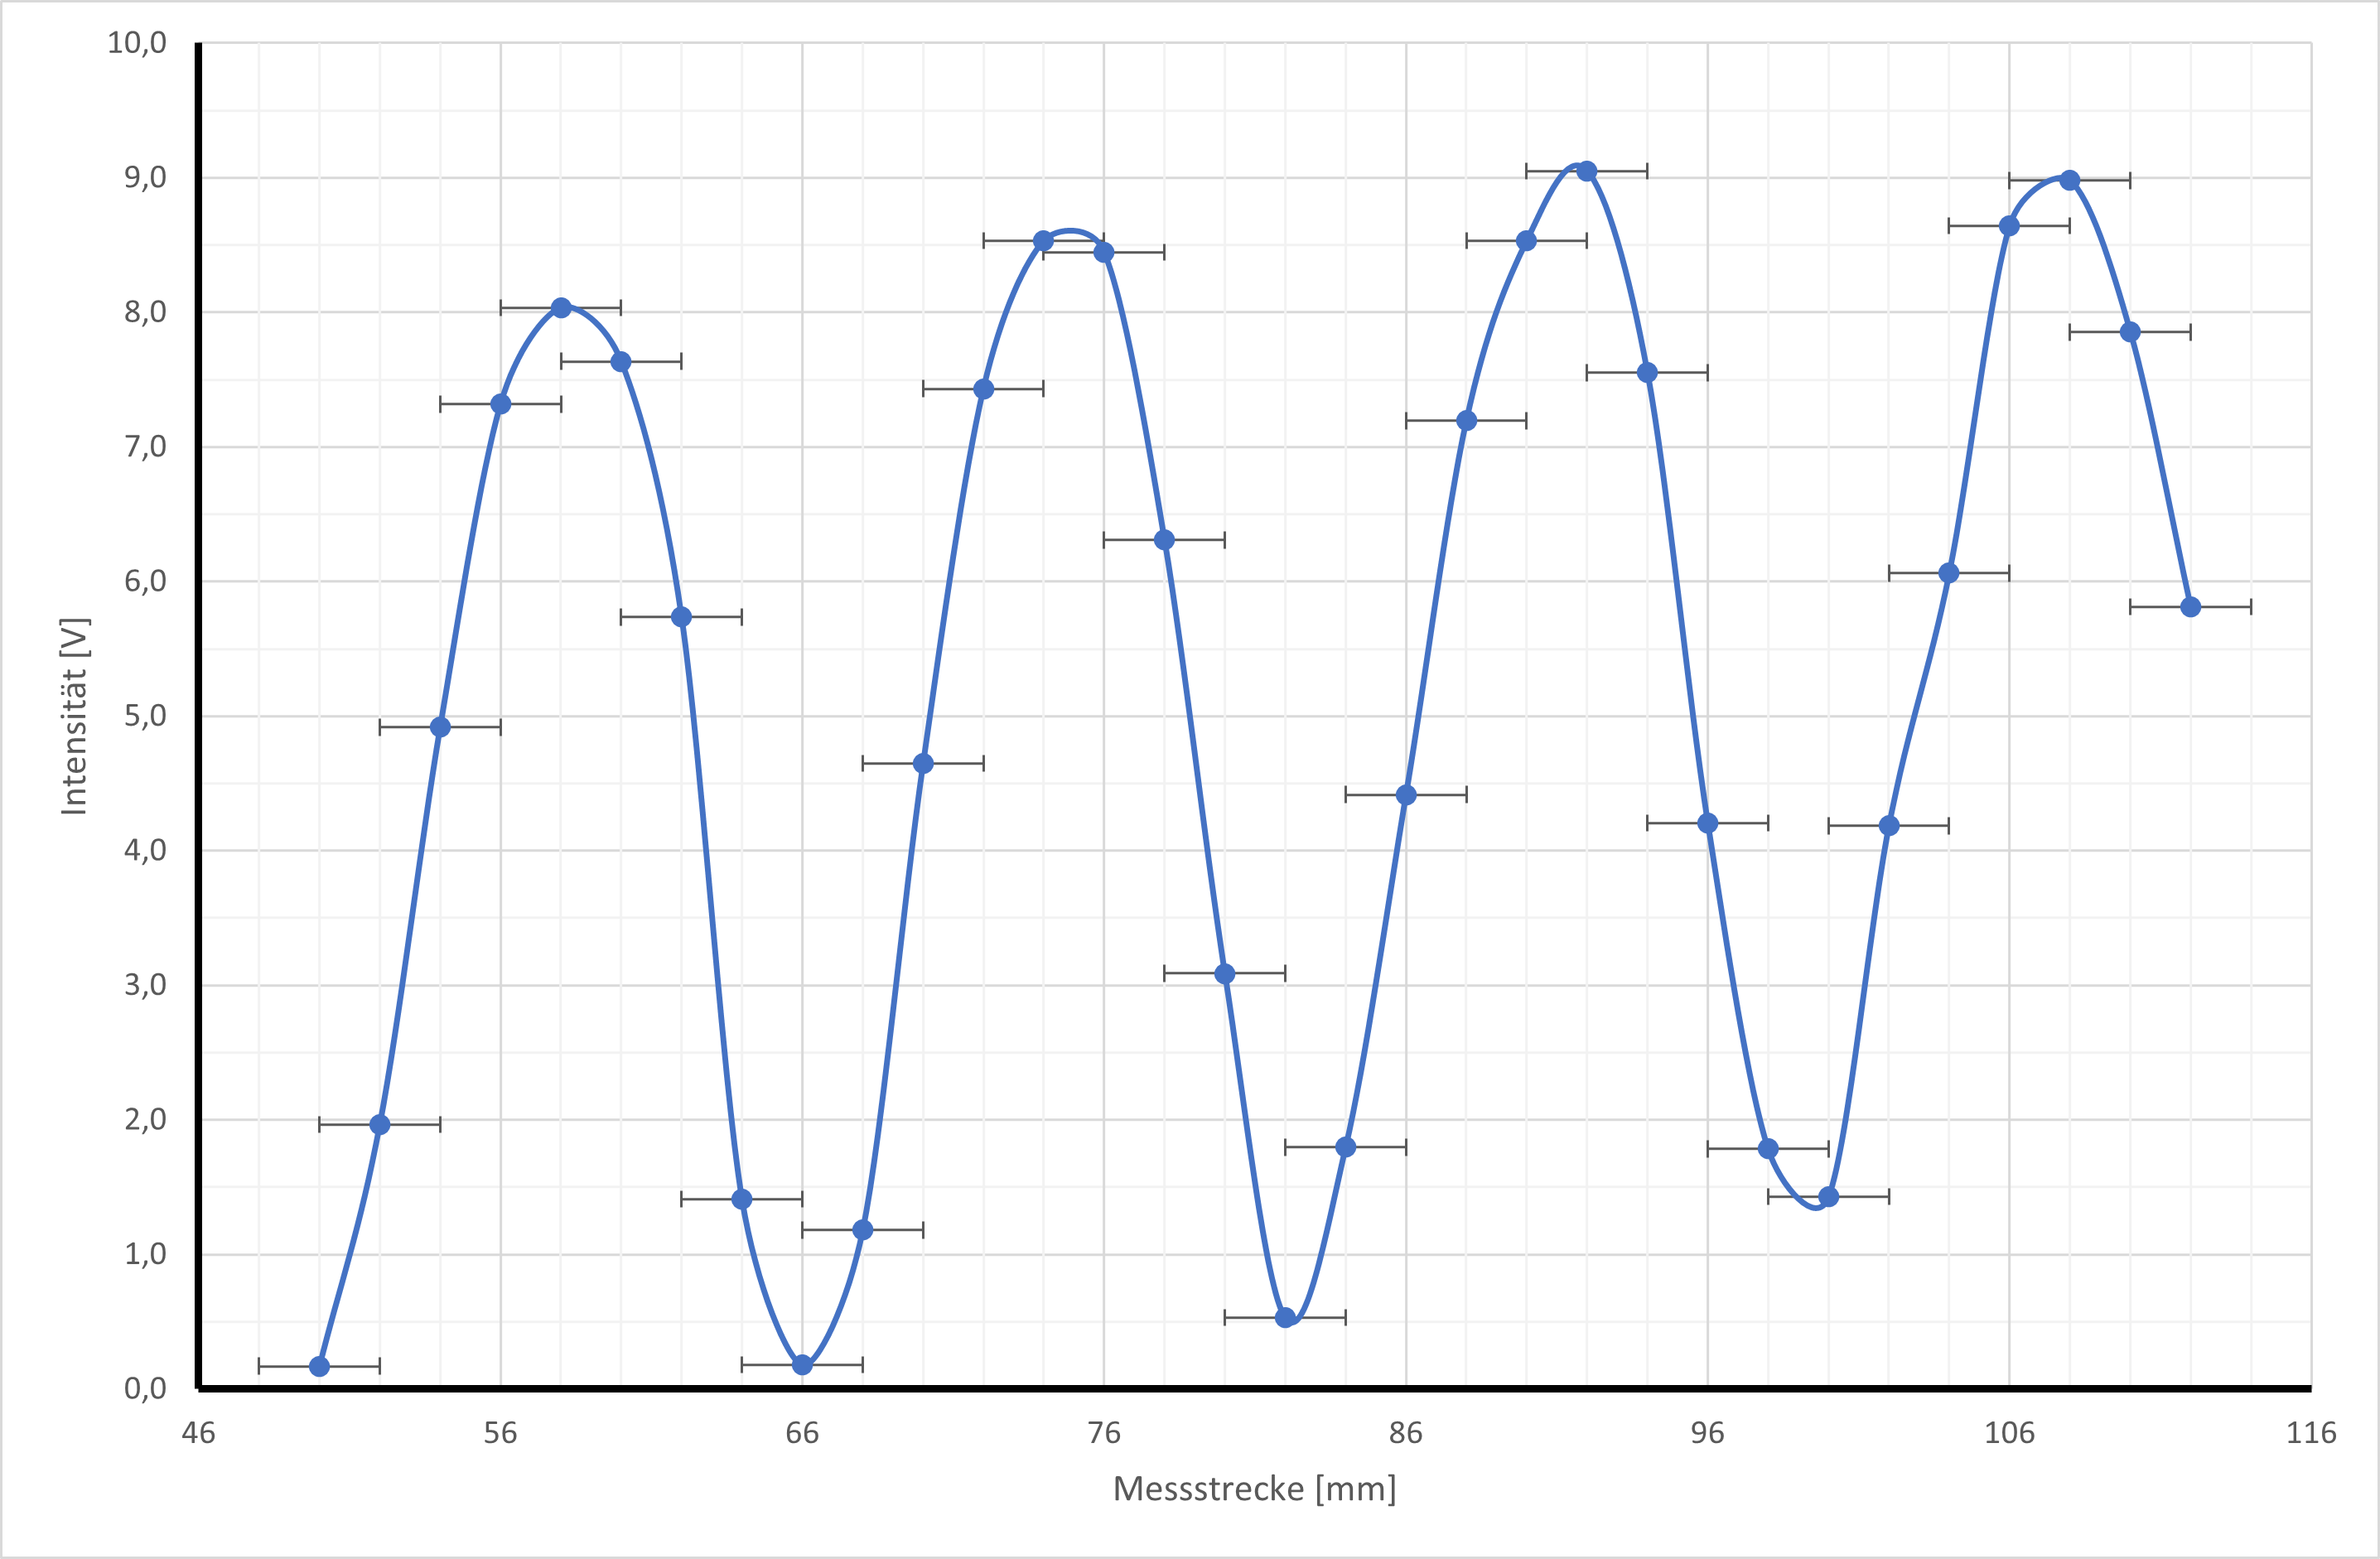
\includegraphics[width=12cm]{Diagramm_Stehende_Wellen}
\centering
\caption{Intensität der Stehenden Welle}
\centering
\label{fig:DiagrammStehendeWelle}
\end{figure}

Die Wellenlänge $\lambda$ wurde in der Tabelle \ref{tab:MesswerteMaxMin} mit Hilfe von Abbildung \ref{fig:DiagrammStehendeWelle} wie folgt bestimmt:

\begin{align}
\lambda = (\text{Minimum} - \text{Maximum}) \cdot 4
\label{eq:lambdaMinMax}
\end{align}
oder:
\begin{align}
\lambda = (\text{Maximum} - \text{Minimum}) \cdot 4
\label{eq:lambdaMaxMin}
\end{align}

Da in den Gleichungen \ref{eq:lambdaMinMax} und \ref{eq:lambdaMaxMin} jeweils der Abstand von einem Maximum zu einem Minimum, was einer halben Periode entspricht, berechnet wird, und die Funktion quadriert ist, muss mit dem Faktor 4 multipliziert werden um $\lambda$ zu berechnen.\\
Die theoretische Herleitung dazu finden Sie in den Häuslichen Vorbereitungen. (Abschnitt \ref{sec:Faktor4})\\

\begin{table}[H]
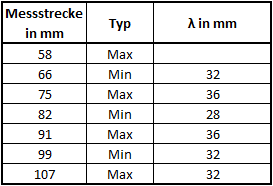
\includegraphics[width=6cm]{Tabelle_Max_Min}
\centering
\caption{Messwerte Max/Min}
\centering
\label{tab:MesswerteMaxMin}
\end{table}

Ermitteln des Mittelwertes der Spalte $\lambda$ aus Tabelle \ref{tab:MesswerteMaxMin} $\pm$ Messunsicherheit mit der Gleichung \ref{eq:Unsicherheit}:

\begin{align*}
\lambda = (32,\overline{6}\pm 2,45854...)\; mm
\end{align*}
Korrekt auf zwei signifikante Stellen gerundet:
\begin{align*}
\lambda = (32,7\pm 2,5)\; mm
\end{align*}
Man erhält die Wellenzahl $k_x$:
\begin{align*}
k_x = \frac{0,192\pm 0,015}{mm}
\end{align*}

\subsection{Beugung am Doppelspalt}
Wie in Abschnitt \ref{sec:runden} beschrieben wurden die Mittelwerte und Messunsicherheiten in Tabelle \ref{tab:MesswerteDoppelspalt} (Abschnitt \ref{sec:MesswerteDoppelspalt}) berechnet und graphisch in Abbildung \ref{fig:DiagrammDoppelspalt} dargestellt.\\
Der Spaltabstand $d$ war beim Versuchsaufbau (siehe Abbildung \ref{fig:AufbauDoppelspalt}) durch die Metallplatte gegeben:

\begin{align*}
d = (90\pm 2)\; mm
\end{align*}

\begin{figure}[H]
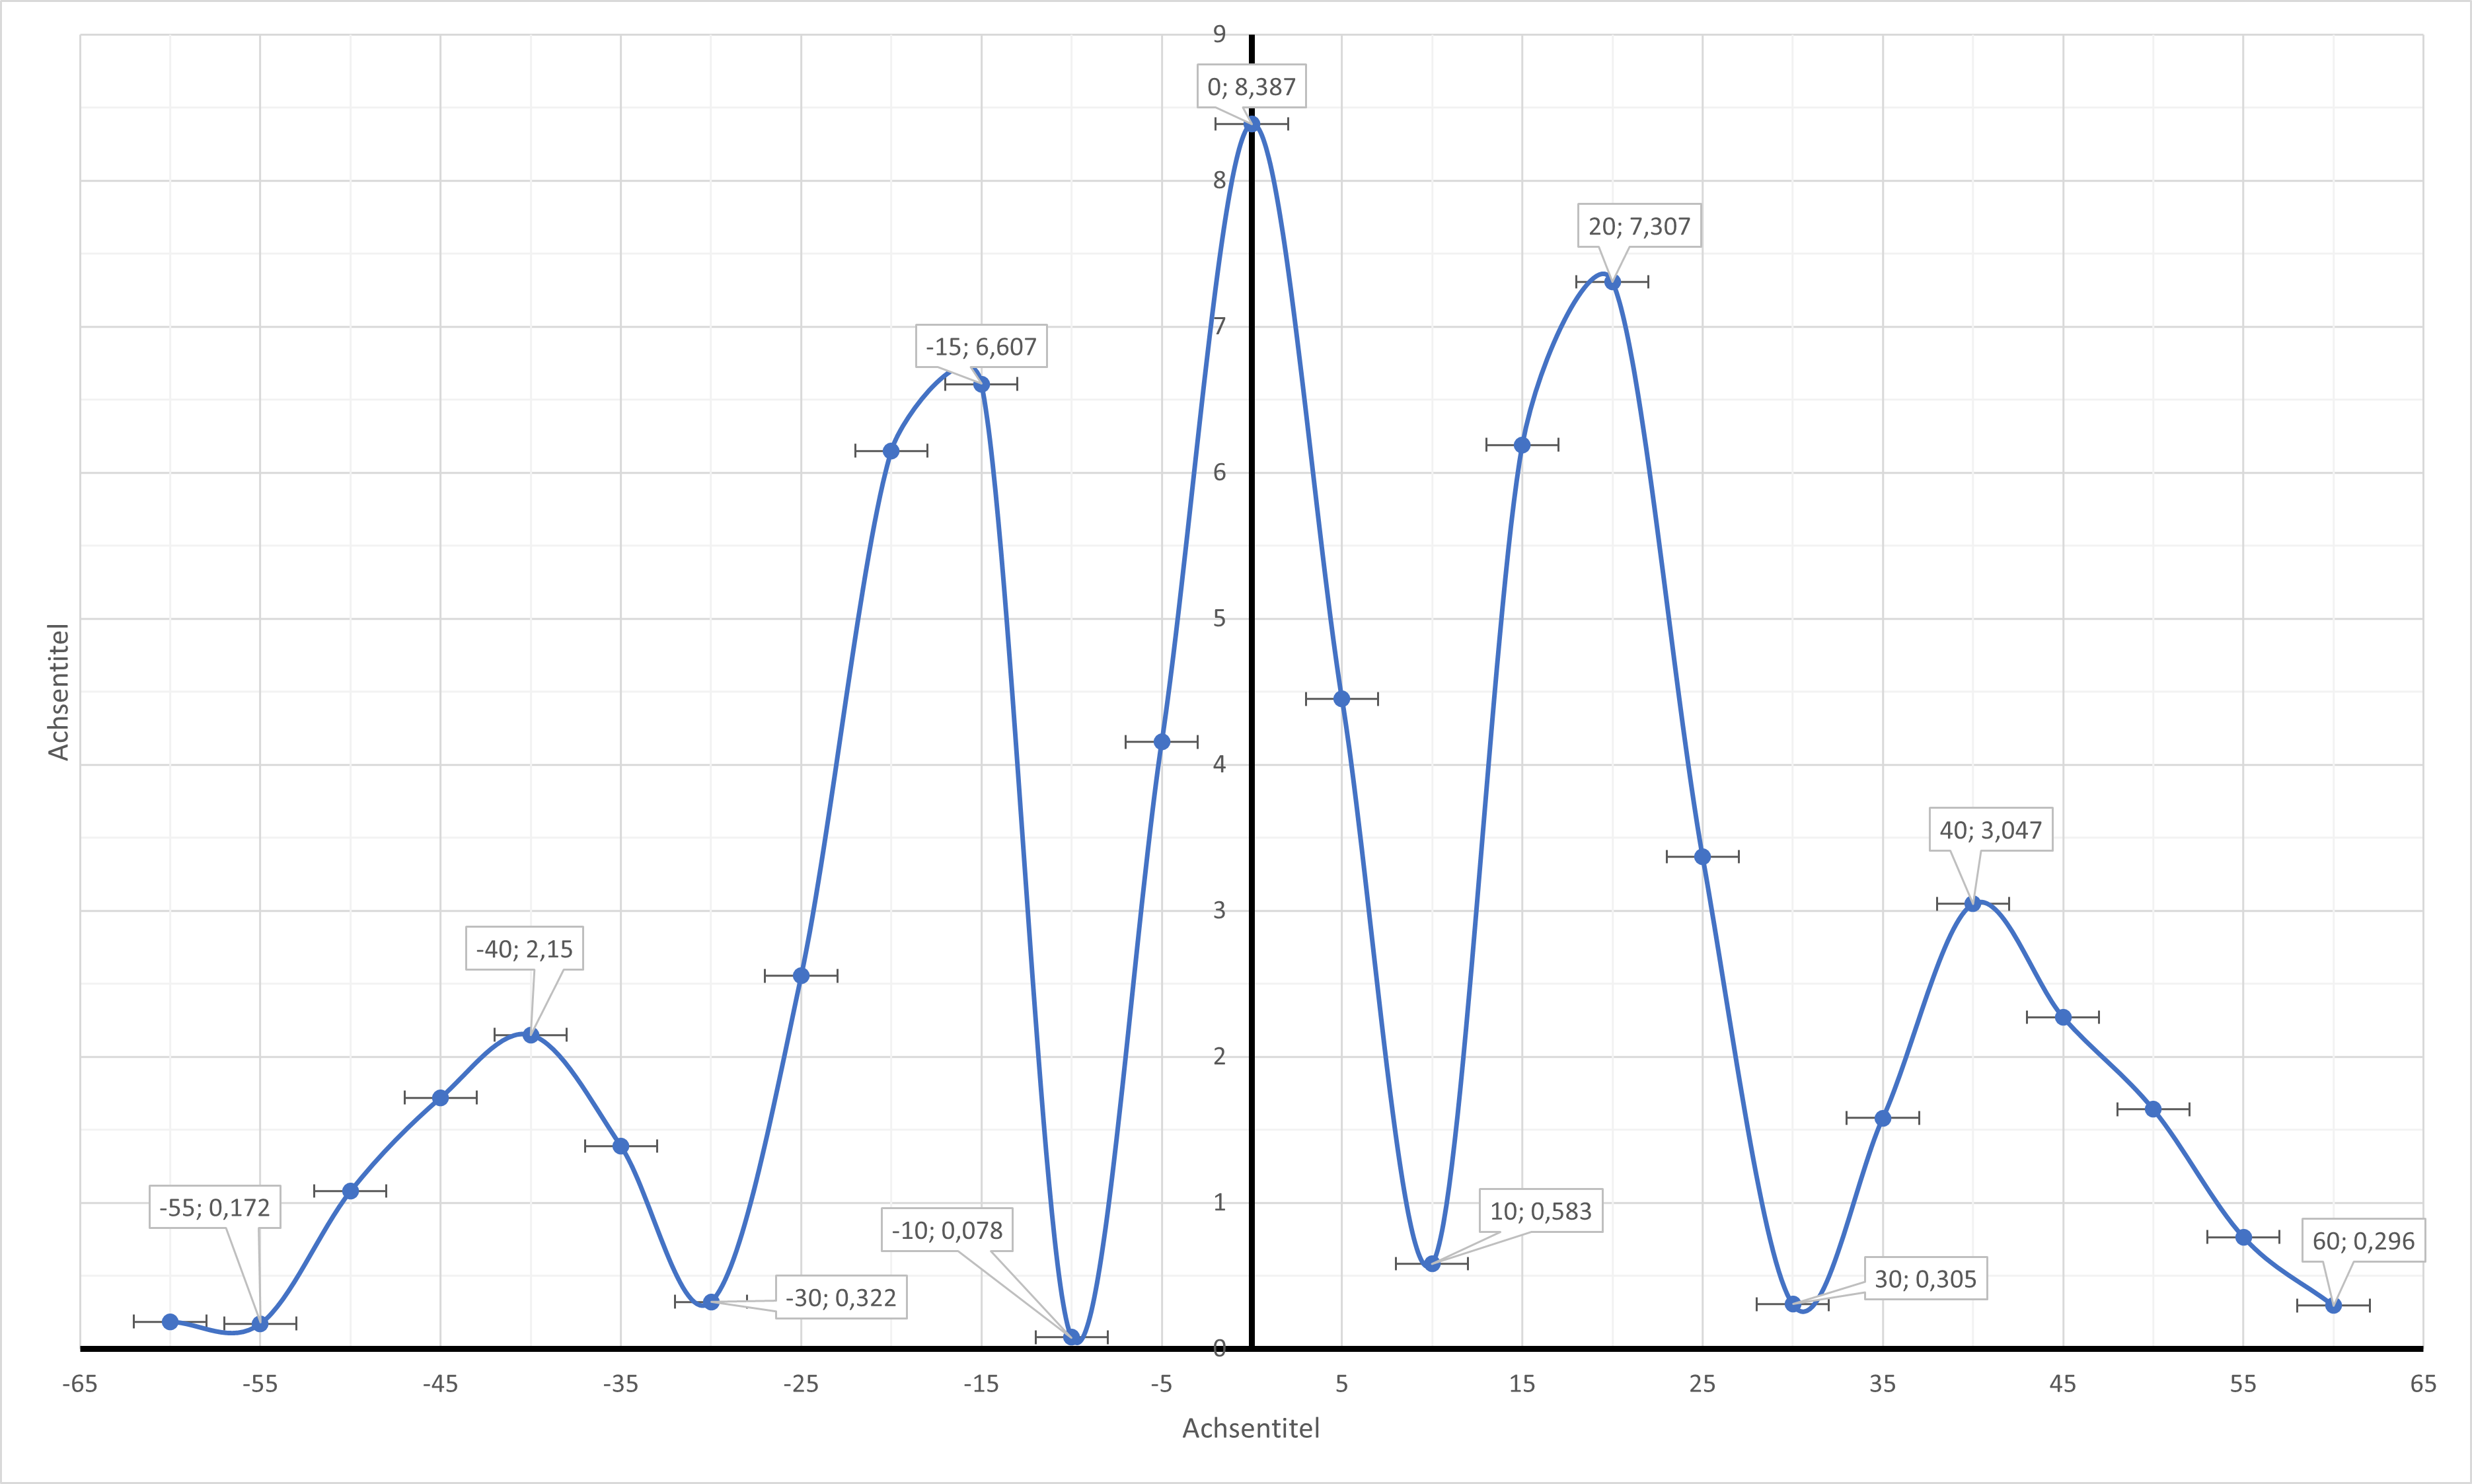
\includegraphics[width=13cm]{Diagramm_Doppelspalt}
\centering
\caption{Intensität der gebeugten Welle nach Doppelspalt}
\centering
\label{fig:DiagrammDoppelspalt}
\end{figure}

In Tabelle \ref{tab:MesswerteMaxMinTheoretisch} wurden die Maxima/Minima mit Hilfe der Gleichungen für konstruktive (\ref{eq:konstruktiveInterferenz}) und destruktive (\ref{eq:destrutiveInterferenz}) Interferenz bestimmt.\\
Für die Berechnung der Messunsicherheit $U_{\theta}$ in Tabelle \ref{tab:MesswerteMaxMinTheoretisch} müssen die Gleichungen \ref{eq:konstruktiveInterferenz} und \ref{eq:destrutiveInterferenz} nach $\theta$ umgestellt und partiell abgeleitet werden.\\
Partielle Ableitungen für konstruktive Interferenz (Gleichung \ref{eq:konstruktiveInterferenz}):
\begin{align}
\frac{\partial \theta}{\partial \lambda} &= \sqrt{\frac{m^2}{d^2-m^2\lambda^2}}\\
\frac{\partial \theta}{\partial d} &= - \sqrt{\frac{m^2 \lambda^2}{d^4-m^2\lambda^2d^2}}
\end{align}
Daraus ergibt sich für Maxima:
\begin{align}
U_{\theta} = (\bigg | \frac{\partial \theta}{\partial \lambda} \bigg | \cdot U_{\lambda} + \bigg | \frac{\partial \theta}{\partial d} \bigg | \cdot U_d) \cdot \frac{180 ^\circ}{\pi}
\end{align}

Partielle Ableitungen für destruktive Interferenz (Gleichung \ref{eq:destrutiveInterferenz}):
\begin{align}
\frac{\partial \theta}{\partial \lambda} &= \sqrt{\frac{(m-\frac{1}{2})^2}{d^2-((2m-1)\cdot \frac{\lambda}{2})^2d^2}}\\
\frac{\partial \theta}{\partial d} &= \sqrt{\frac{(\lambda m-\frac{1}{2})^2}{d^4-((2m-1)\cdot \frac{\lambda}{2})^2d^2}}\\
\end{align}
Daraus ergibt sich für Minima:
\begin{align}
U_{\theta} = (\bigg | \frac{\partial \theta}{\partial \lambda} \bigg | \cdot U_{\lambda} + \bigg | \frac{\partial \theta}{\partial d} \bigg | \cdot U_d) \cdot \frac{180 ^\circ}{\pi}
\end{align}

\begin{table}[H]
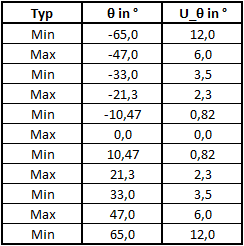
\includegraphics[width=6cm]{Tabelle_maxmin_theoretisch}
\centering
\caption{Messwerte Max/Min Doppelspalt}
\centering
\label{tab:MesswerteMaxMinTheoretisch}
\end{table}


\newpage

\section{Wertung/Fazit}
\subsection{Stehende Wellen}
Bei der Durchführung des Versuches ließen sich die charakteristischen Eigenschaften einer stehenden Welle deutlich erkennen. Es gab jedoch einige Fehlerquellen wodurch unsere Messwerte von den theoretischen Werten abweichen. Unsere Messunsicherheit für den Abstand der Feldsonde zur Metallplatte $U_s = 1,5$ mm. (Positionierungsungenauigkeit)
Da wir nur einen Messwert pro Stelle gemessen haben, gibt es einen Einfluss zufälliger Messabweichungen. Würde man mehr Messwerte aufnehmen, wäre die Standardabweichung kleiner und das Ergebnis genauer.
Außerdem wurde die Kurve (siehe Abbildung \ref{fig:DiagrammStehendeWelle}) automatisch von Excel geglättet (interpoliert). Es ist nicht klar wie stark Excel geglättet hat.
Zudem gibt es eine Ungenauigkeit beim Ablesen der Wellenlänge aus dem Diagramm.
(siehe Tabelle \ref{tab:MesswerteMaxMin})\\
Wenn man die Theorie betrachtet, müssten die Abstände zwischen den Extrema immer gleich weit sein. Außerdem müsste die Amplitude der Extrema immer gleich hoch sein. Dies ist bei unseren Messungen nicht der Fall (siehe Abbildung \ref{fig:DiagrammStehendeWelle})
Wenn man allerdings die Messungenauigkeit abzieht und mit einberechnet, dass es keine optimalen Bedingungen waren (kein Vakuum) ist das Ergebnis zufriedenstellend.

\subsection{Beugung am Doppelspalt}
Bei diesem Versuch ließen sich die Intensitätsverteilungen durch Beugung am Doppelspalt gut erkennen. Jedoch gab es auch bei diesem Versuch deutliche Abweichungen von der Theorie. Die Maxima mit den Ordnungzahlen $m = +1$ und $m = -1$ sollten die selbe Intensität aufweisen. Dies ist in unserem Diagramm (siehe Abbildung \ref{fig:DiagrammDoppelspalt}) nicht der Fall. Hier gibt es ähnliche Fehlerquellen wie beim ersten Versuchsteil. Auch hier wurde die Kurve von Excel geglättet. Ebenfalls gab es eine Positionierungsungenauigkeit $U_{\theta} = 2 ^\circ$. In diesem Versuchsteil wurden zumindest drei Werte pro Messung genommen. Trotzdem ist die Anzahl der Messung noch viel zu gering um zufällige Messfehler ausschließen zu können.
Allerdings kann man auch hier, wenn man die Messungenauigkeit abzieht mit den Ergebnissen zufrieden sein.

\newpage
\section{Anhang}
\subsection{Messwerte Stehende Wellen}
\label{sec:MesswerteStehendeWellen}
\begin{table}[H]
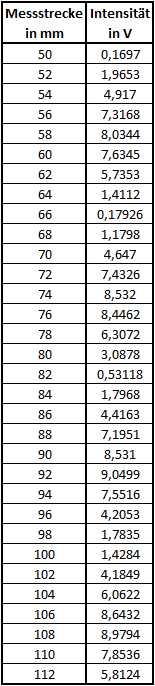
\includegraphics[width=4cm]{Messwerte_Stehende_Wellen}
\centering
\caption{Messwerte Stehende Wellen}
\label{tab:MesswerteStehendeWellen}
\end{table}

\subsection{Messwerte Beugung am Doppelspalt}
\label{sec:MesswerteDoppelspalt}
\begin{table}[H]
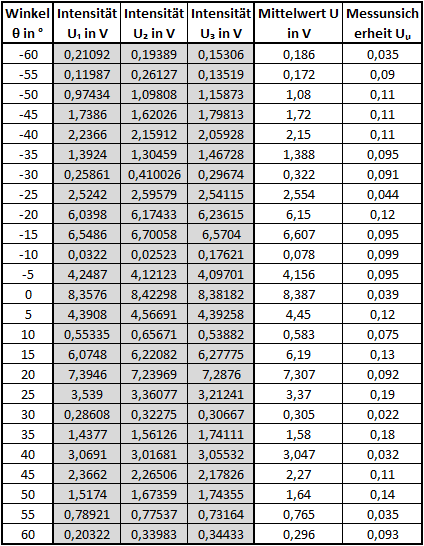
\includegraphics[width=12cm]{Messwerte_Doppelspalt}
\centering
\caption{Messwerte Beugung am Doppelspalt}
\label{tab:MesswerteDoppelspalt}
\end{table}
\subsection{Skizze Aufbau - Stehende Wellen}

\label{sec:SkizzeStehendeWellen}

\begin{figure}[H]
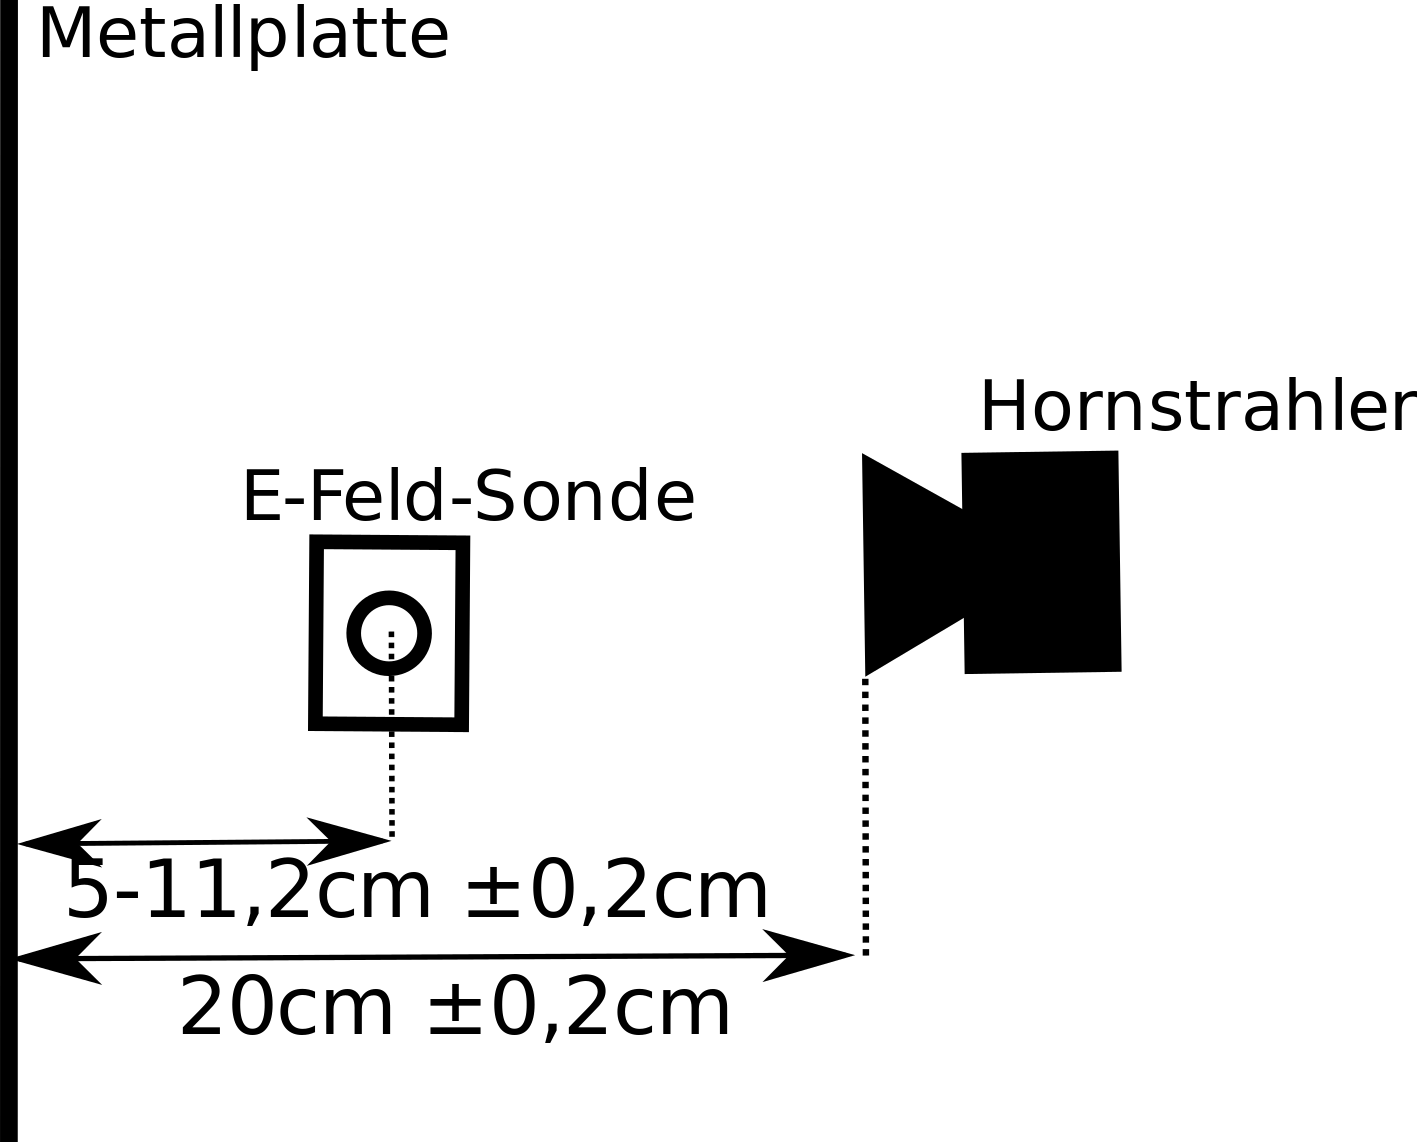
\includegraphics[width=8cm]{Zeichnung_Wellen}
\centering
\caption{Skizze Aufbau - Stehende Wellen}
\centering
\label{fig:SkizzeStehendeWellen}
\end{figure}

\subsection{Skizze Aufbau - Beugung am Doppelspalt}

\label{sec:SkizzeDoppelspalt}

\begin{figure}[H]
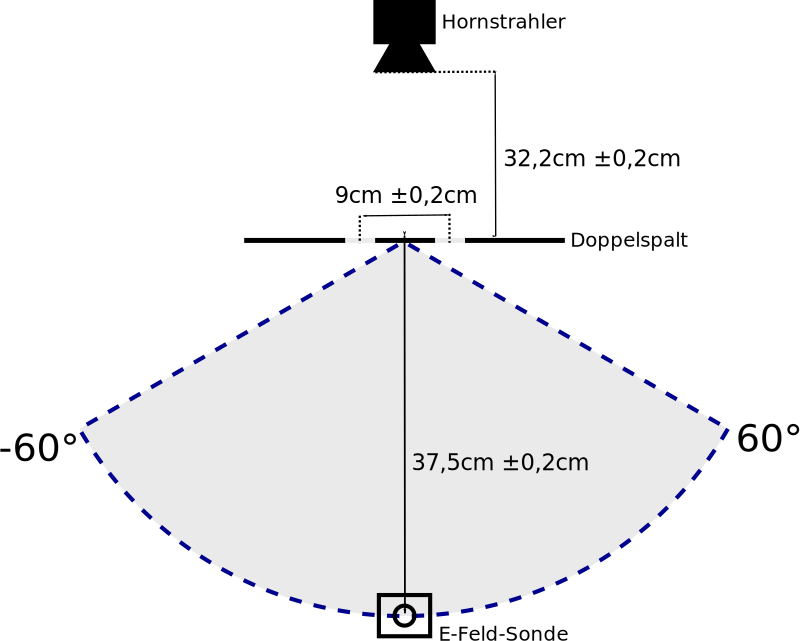
\includegraphics[width=12cm]{Zeichnung_Doppelspalt}
\centering
\caption{Skizze Aufbau - Beugung am Doppelspalt}
\centering
\label{fig:SkizzeDoppelspalt}
\end{figure}

\newpage
\section{Literatur}
$[$1$]$ Skript: Versuch 2.2 - Stehende Wellen und Beugung am Doppelspalt \\
$[$2$]$ Vorlesungsfolien: 1. Semester Physik, Herr Prof. Kaloudis \\
$[$3$]$ Hering, Ekbert ; Martin, Rolf ; Stohrer, Martin: Physik für Ingenieure. Springer-Verlag \\
$[$4$]$ Abbildung~\ref{fig:skizzeDoppelspalt}: Skizze - Beugung am Doppelspalt von \href{http://aviacia.info/p/beugung-am-gitter-4265}{http://aviacia.info} (08.04.2022)\\
$[$5$]$ Formeln + Hilfen Höhere Mathematik, G.Merziger; G.Mühlbach; D.Wille; T.Wirth, Binomi Verlag (8. Auflage)


\label{LastPage}

\end{document}
%%% Local Variables:
%%% mode: latex
%%% TeX-master: t
%%% End:
